% !TEX root=../../Thesis.tex
\chapter{Introduction} \label{ch:intro}
The way of transportation is currently evolving, and autonomous driving technology is expected to have a big impact on this transformation~\cite{traffic21}. Over one million people are killed in traffic-related accidents each year, where the vast majority of the accidents are caused by human mistakes~\cite{WHO2018, NHTSA2018}. By helping humans with perception, prediction and decision making autonomous driving could significantly improve traffic safety and make way for new innovative road infrastructure. Without the requirement of a present human for each transportation vehicle, the efficiency of traffic can be improved by scheduling commercial transports outside of rush hours~\cite{FAGNANT2015167}. Number of parking spots in cities can be reduced if the vehicle can autonomously drive itself to a less crowded area when not in use and drive itself back when needed. Congestion and traffic jams could also be reduced if a large amount of vehicles in traffic are autonomous and optimize around the same goal e.g., traffic flow or fuel efficiency. 

%\todo{Level 2: Volvo pilot assist and tesla auto pilot. Level 4: Waymo. Woven automated city}

Thanks to the rapid success of machine learning during the last decades, major progress towards deploying autonomous vehicles in the real world. One clear benefactor of the new machine learning technics are the perception systems~\cite{Janai2020}. Better perception enables more accurate representation of the environment. 
% The low-level control of the vehicle is a mature research area and can be solved with classical control theory methods~\cite{Paden2016}.
However, for complex scenarios such as urban intersections and roundabouts with dense traffic remain challenging for autonomous vehicles because it requires a higher level of interaction between road users. 
When a human driver approach an intersection, it is natural to observe the environment to identify the traffic light, signs and other approaching vehicles. Then assess the situation to find out \textit{who has the right of way?} Before deciding weather to  drive or yield. 
If all drivers could perfectly assess the situation and follow the right of way, there would be no accidents or collisions. However, according to the Insurance Institute for Highway Safety~\cite{IIHS2019}, in 2019, an estimated \num{115741} people were injured by drivers running a red light and \num{928} of them were killed. 
This motivates the development of control algorithms for autonomous vehicles which can take into account other drivers intention and at the same time behave in a ``human-like'' way. 


This thesis presents \gls{rl} methods for generating efficient and scalable decision strategies for autonomous vehicles driving in environments with other drivers and their intentions are not observable. Starting with introducing the different \gls{ad} levels in Section~\ref{sec:intro_ad}.
Section~\ref{sec:intro_intersections} defines the terms' scenario, intersection and intention used in this thesis.
\Citet{Shalev2016} raises two concerns when using Machine learning, specially Reinforcement learning, for autonomous driving applications: ensuring functional safety of the driving policy and that the \gls{mdp} model is problematic, because of unpredictable behavior of other drivers. 
Ensuring functional safety is not the main focus of this work, but because of its importance, it is briefly addressed in Section~\ref{sec:system_architecture} together with a proposed system architecture that can utilize the work presented in this thesis in a safe way. 
The handling of the unpredictable behavior of other drivers is the main topic in this thesis and the research questions are presented in Section~\ref{sec:research_questions}. The scope and limitations are listed in Section~\ref{sec:scope}. Finally, the contributions of this thesis is presented in Section~\ref{sec:contributions}. 

\section{Autonomous Driving}
\label{sec:intro_ad}
When talking about autonomous driving, it is first important to specify which level of autonomy that is being discussed. The Society of Automotive Engineers has classified these different levels of autonomy ranging from zero to five~\cite{SAE2021}, also referred to as L0-L5. L0 is a vehicle with no autonomy, whereas a fully autonomous vehicle that can operate in any environment and without any human supervision is defined as L5. Popular \gls{adas} functions today, like Tesla autopilot and the Volvo Pilot Assist, are classified as level 2, with the main criteria being that the driver is in control and is supported by the system. This puts a requirement on the driver to always supervise the vehicle and take over when needed to maintain safety. For L3 and higher the responsibility of driving is on the system. At L3 the driver still has to take control over the vehicle but at the request of the system, and at L4 and L5 the autonomous driving features no longer require the driver to take over. Finally, the main difference between L4 and L5 is the capability of driving anywhere, under all conditions. 

% Another way to categorize these autonomy levels is: supervised and unsupervised driving. Supervised driving include L0-L3 where the driver has to supervise the system and take control when necessary, while unsupervised 
% \tommy{Level 2: You are diving, provide steering and breaking support to the driver, lane centering and adaptive cruise control}
The methods presented in this thesis are aimed at an autonomy level between L3 and L5. At this level the system is expected to handle all aspects of driving within a specific task such as crossing an intersection. 

In this thesis, the automated vehicle making the decisions are referred to as the ego vehicle.
Other traffic participants are assumed to be vehicles driven by other human drivers but could be extended to pedestrians bicyclist and other autonomous vehicles. 


\subsection{Scenarios and unsignalized intersections}
\label{sec:intro_intersections}
% When a pedestrian approach a crossing they have been taught at a young age to look at both sides of the road before crossing. The same apply for a human driver approaching an intersection. 
% When a human driver approach an intersection, it is natural to observe the environment to identify the traffic light, signs and other approaching vehicles. Then assess the situation, who has the right of way? 

% The intention of the other driver can be guided by the 
% Recently nontraditional intersections are also becoming increasingly popular. The goal of these designs is to reduce the number and/or severity of conflict points by altering the customary vehicular paths at the intersection. In light of the increased focus on and occurrence of these intersection types, it is expected that the application of nontraditional designs will continue to spread.

\begin{figure}[h]
	\centering
	\begin{subfigure}[t]{0.48\columnwidth}
		\centering
		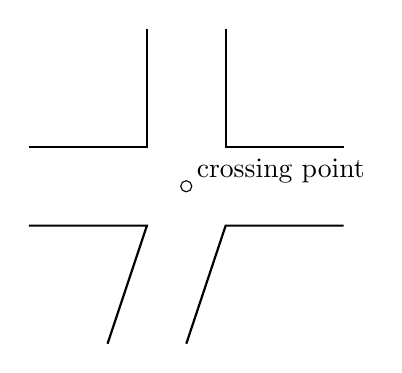
\begin{tikzpicture}
			% Crossing
			\def\crossleftx{-2}
			\def\crossrightx{2}
			\def\crosstopy{2}
			\def\crossboty{-2}
			\def\roadwidth{0.5}

			\draw (0,0) circle (2pt);
			\node at (1.2, 0.2) {crossing point};
			\draw[thick] (\crossleftx, \roadwidth) -- (-\roadwidth, \roadwidth) -- (-\roadwidth, \crosstopy);
			\draw[thick] (\crossleftx, -\roadwidth) -- (-\roadwidth, -\roadwidth) -- (-\roadwidth-\roadwidth, \crossboty);
			\draw[thick] (\roadwidth, \crosstopy) -- (\roadwidth, \roadwidth) -- (\crossrightx, \roadwidth);
			\draw[thick] (\roadwidth-\roadwidth, \crossboty) -- (\roadwidth, -\roadwidth) -- (\crossrightx, -\roadwidth);
		\end{tikzpicture}
		\caption{Single intersection}
\end{subfigure}%
	~ 
	\begin{subfigure}[t]{0.48\columnwidth}
		\centering
		\begin{tikzpicture}
			% Crossing
			\def\crossleftx{-2.5}
			\def\crossrightx{2.5}
			\def\crosstopy{2}
			\def\crossboty{-2}
			\def\roadwidth{0.5}

			\draw (-0.5,0) circle (2pt);
			\draw (0.5,0) circle (2pt);
			% \node at (0.7, 0.2) {crossing point$^1$};
			\draw[thick] (\crossleftx, \roadwidth) -- (-\roadwidth-0.5, \roadwidth) -- (-\roadwidth-0.5, \crosstopy);
			\draw[thick] (\crossleftx, -\roadwidth) -- (-\roadwidth-0.5, -\roadwidth) -- (-\roadwidth-0.5, \crossboty);
			\draw[thick] (0, \crosstopy) -- (0, \roadwidth);
			\draw[thick] (0, -\roadwidth) -- (0, \crossboty);
			\draw[thick] (\roadwidth+0.5, \crosstopy) -- (\roadwidth+0.5, \roadwidth) -- (\crossrightx, \roadwidth);
			\draw[thick] (\roadwidth+0.5, \crossboty) -- (\roadwidth+0.5, -\roadwidth) -- (\crossrightx, -\roadwidth);
		\end{tikzpicture}
		\caption{Double intersection}
	\end{subfigure}

	\caption{Examples of different intersections}
	\label{fig:example_intersections}

\end{figure}
In this thesis there is a separation between scenario and intersection. An intersection refers the geometrical shape of the intersection, like number of junctions, conflict points, turns and angle of incidence, as shown in Figure~\ref{fig:example_intersections}. While a scenario is defined as the combination of an intersection, its' traffic participants, their intentions, positions and velocities, as shown in Figure~\ref{fig:example_scenarios}. 
An unsignalized intersection is defined as any junction of two or more roads where the right-of-way for a car, bicycle and pedestrian is not controlled by a regulatory (i.e., STOP or YIELD) sign or a traffic signal.

More detail on the specific intersections and scenarios considered in this work is presented in Chapter~\ref{ch:modeling_intersection}.

\begin{figure}[h]
	\centering
	\begin{subfigure}[t]{0.48\columnwidth}
		\centering
		\begin{tikzpicture}
			% Crossing
			\def\crossleftx{-2}
			\def\crossrightx{2}
			\def\crosstopy{2}
			\def\crossboty{-2}
			\def\roadwidth{0.5}

			\draw (0,0) circle (2pt);
			\node at (1.2, 0.2) {crossing point};
			\draw[thick] (\crossleftx, \roadwidth) -- (-\roadwidth, \roadwidth) -- (-\roadwidth, \crosstopy);
			\draw[thick] (\crossleftx, -\roadwidth) -- (-\roadwidth, -\roadwidth) -- (-\roadwidth, \crossboty);
			\draw[thick] (\roadwidth, \crosstopy) -- (\roadwidth, \roadwidth) -- (\crossrightx, \roadwidth);
			\draw[thick] (\roadwidth, \crossboty) -- (\roadwidth, -\roadwidth) -- (\crossrightx, -\roadwidth);

			% 	cars
			\node[inner sep=0pt] (ego_car) at (\crossleftx+0.5,0)
			{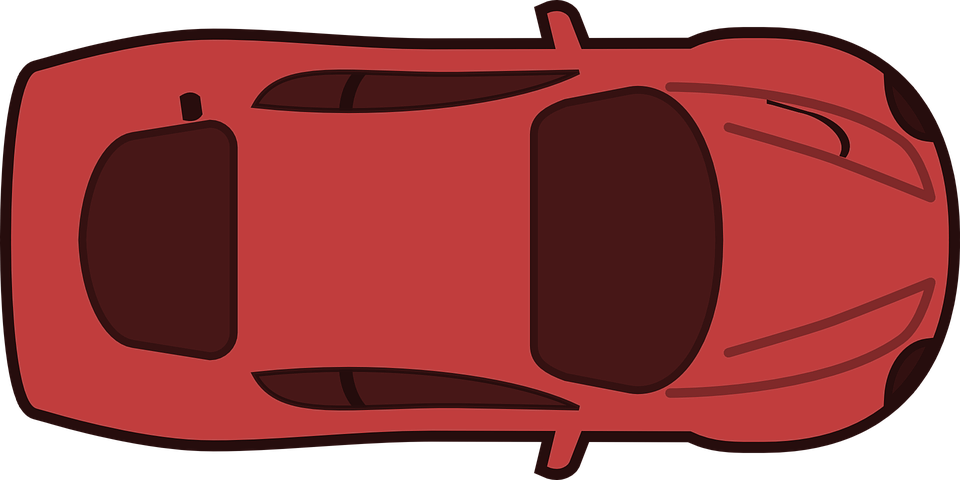
\includegraphics[width=.18\textwidth, angle=0]{figures/ego_car_top_down.png}};

			\node[inner sep=0pt] (target_car) at (0,\crosstopy-0.5)
			{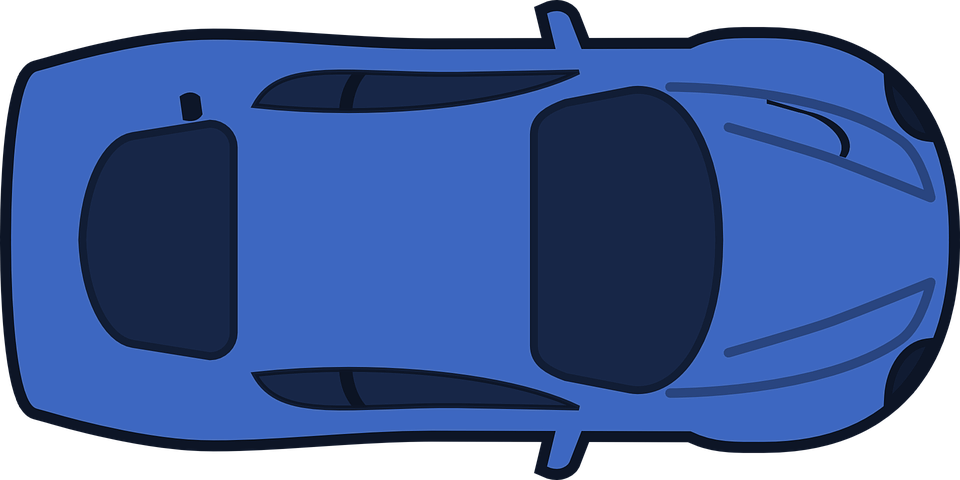
\includegraphics[width=.18\textwidth, angle=-90]{figures/target_car_top_down.png}};

			%  \node[inner sep=0pt] (targetcar2) at (0,2.5)
			%  {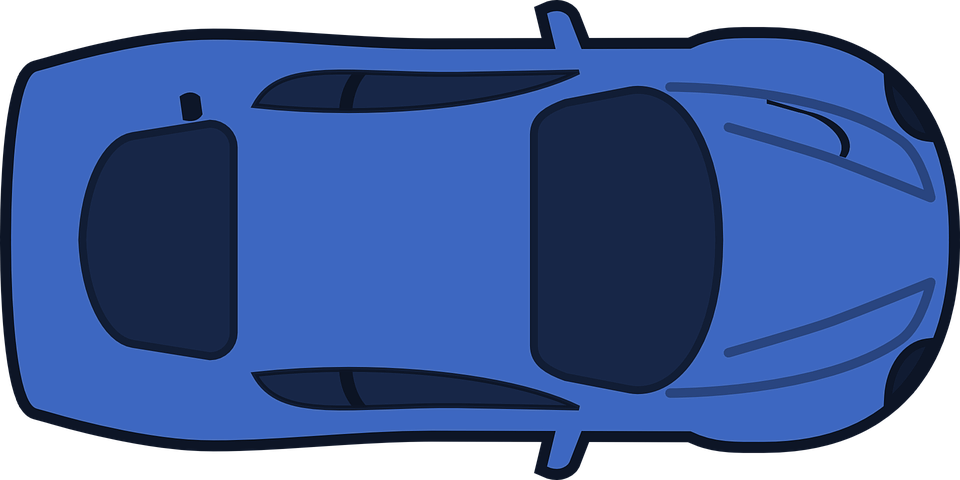
\includegraphics[width=.18\textwidth, angle=-90]{figures/target_car_top_down.png}};
			%  \node (tctext2) [right=of targetcar2] {Car 2};
			
			% \node[inner sep=0pt] (target_car_1) at (0,-1.5)
			% {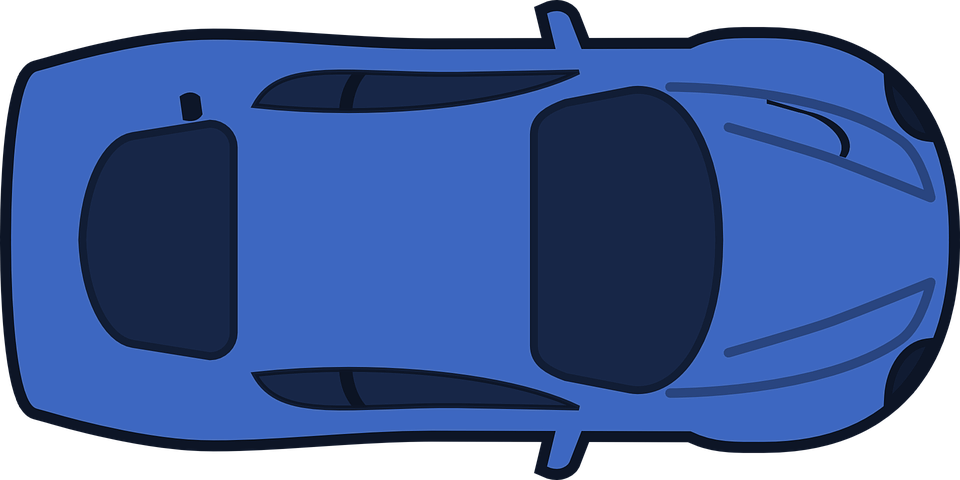
\includegraphics[width=.18\textwidth, angle=-90]{figures/target_car_top_down.png}};
			% \node (tc_text1) [right=of target_car_1] {Car 1};
		\end{tikzpicture}
		\caption{Single intersection scenario}
\end{subfigure}%
	~ 
	\begin{subfigure}[t]{0.48\columnwidth}
		\centering
		\begin{tikzpicture}
			% Crossing
			\def\crossleftx{-2.5}
			\def\crossrightx{2.5}
			\def\crosstopy{2}
			\def\crossboty{-2}
			\def\roadwidth{0.5}

			\draw (-0.5,0) circle (2pt);
			\draw (0.5,0) circle (2pt);
			% \node at (0.7, 0.2) {crossing point$^1$};
			\draw[thick] (\crossleftx, \roadwidth) -- (-\roadwidth-0.5, \roadwidth) -- (-\roadwidth-0.5, \crosstopy);
			\draw[thick] (\crossleftx, -\roadwidth) -- (-\roadwidth-0.5, -\roadwidth) -- (-\roadwidth-0.5, \crossboty);
			\draw[thick] (0, \crosstopy) -- (0, \roadwidth);
			\draw[thick] (0, -\roadwidth) -- (0, \crossboty);
			\draw[thick] (\roadwidth+0.5, \crosstopy) -- (\roadwidth+0.5, \roadwidth) -- (\crossrightx, \roadwidth);
			\draw[thick] (\roadwidth+0.5, \crossboty) -- (\roadwidth+0.5, -\roadwidth) -- (\crossrightx, -\roadwidth);

			% 	cars
			\node[inner sep=0pt] (ego_car) at (\crossleftx+0.5,0)
			{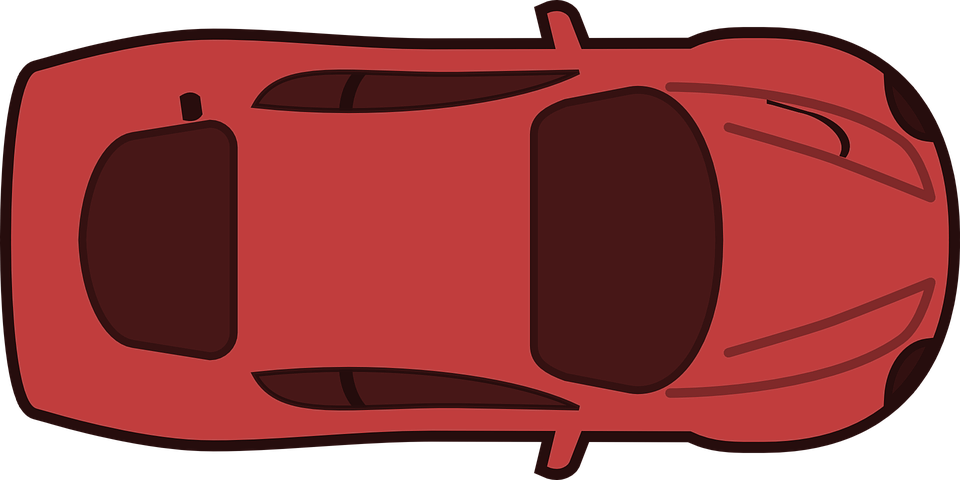
\includegraphics[width=.18\textwidth, angle=0]{figures/ego_car_top_down.png}};

			\node[inner sep=0pt] (target_car) at (-0.5,\crosstopy-0.5)
			{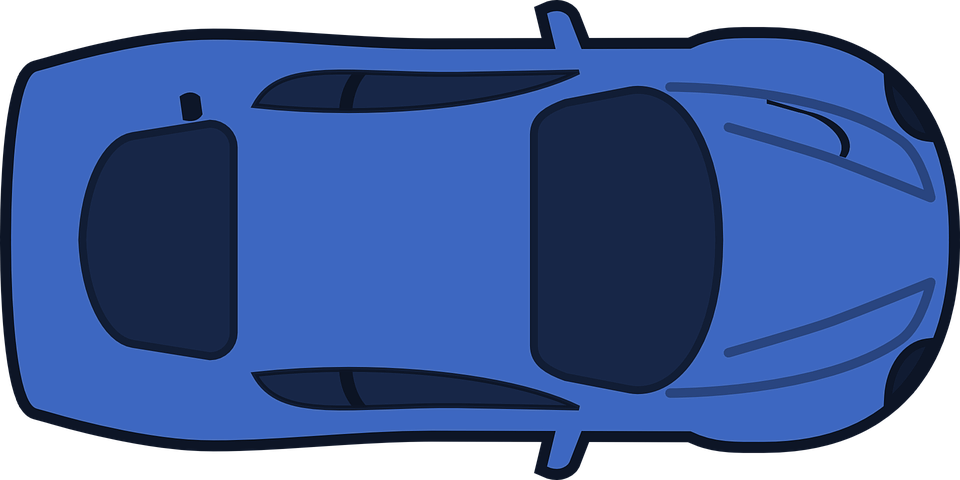
\includegraphics[width=.18\textwidth, angle=-90]{figures/target_car_top_down.png}};

			\node[inner sep=0pt] (target_car_2) at (0.5,\crossboty+0.5)
			{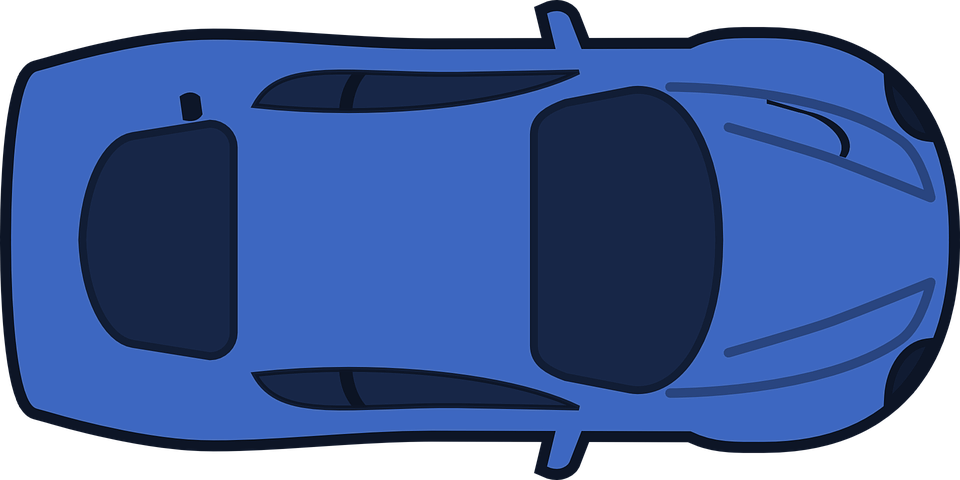
\includegraphics[width=.18\textwidth, angle=90]{figures/target_car_top_down.png}};
		\end{tikzpicture}
		\caption{Double intersection scenario}
	\end{subfigure}

	\caption{Examples of different scenarios}
	\label{fig:example_scenarios}

\end{figure}

\tommy{what I want to say here is: define an unsignalized intersection. There are many variations. Roundabouts are defined as unsignalized intersection. To satisfy the requirement of being able to drive anywhere for level 5 it is necessary to find a method that can scale to these different scenarios}

%  In light of the increased focus on and occurrence of these intersection types nationwide, it is expected that the application of nontraditional designs will continue to spread.

\section{System architecture}
\label{sec:system_architecture}
The architecture of an autonomous driving system can be divided into perception, planning and control~\cite{Schwarting2018,Kortenkamp2008}.

The perception module is responsible for sensing and mapping the environment with the use of sensors such as LIDARs, cameras, radars etc. The raw data from the sensors are then processed though various sensor fusion techniques to generate a representation of the environment, e.g., position, velocity of other traffic participants while also describing the road such as width and distance to the next intersection. This information is then used by the planner to create a driving strategy of how to transverse through the world. However, the information from the sensors are often noisy, with false positives and false negatives making it difficult for the planner.

Tactical planning can be divided into three categories, the proactive, active and reactive. A proactive module would be something like a precautionary safety module that interprets the information about the environment and create constraints that is sent to the active planner, like  driveable area, allowed speeds and actions. These constraints are generated from a set of safety goals and rules, making this the first layer of protection that can ensure safety. 
The role of the active planner is to take this sets of allowed actions and prescribe the behavior of the vehicle through decisions such as drive, yield or stop. The goal of these high level decisions is to optimize metrics such as comfort, fuel consumption and time to goal. These decisions are then sent to a motion planner that generates a safe dynamically feasible path for the vehicle for a shorter planning horizon of around $0.1$s. 
At the same time, a reactive, collision avoidance, module make sure that the chosen decision and path does lead to any collisions. Unlike the decision maker, the collision avoidance module main goal is to identify imminent danger and therefore has access to more aggressive actions like emergency breaking to ensure safety. 
 
In the industry today the main standard for functional safety in motorized vehicles is the ISO 26262 standard, titled "Road vehicles – Functional safety"~\cite{ISO26262}. It uses a \gls{asil} to classify the inherent safety risk in an automotive system and the functions or modules of such a system. The \gls{asil} classification is used to express the level of risk reduction required to prevent a specific hazard, from \gls{asil} D to \gls{asil} A. \gls{asil} D represents the highest hazard level and \gls{asil} A the lowest. There is a level with no safety relevance and only standard Quality Management processes are required, this level is referred to as QM.

\begin{figure}[h]
	\centering
	 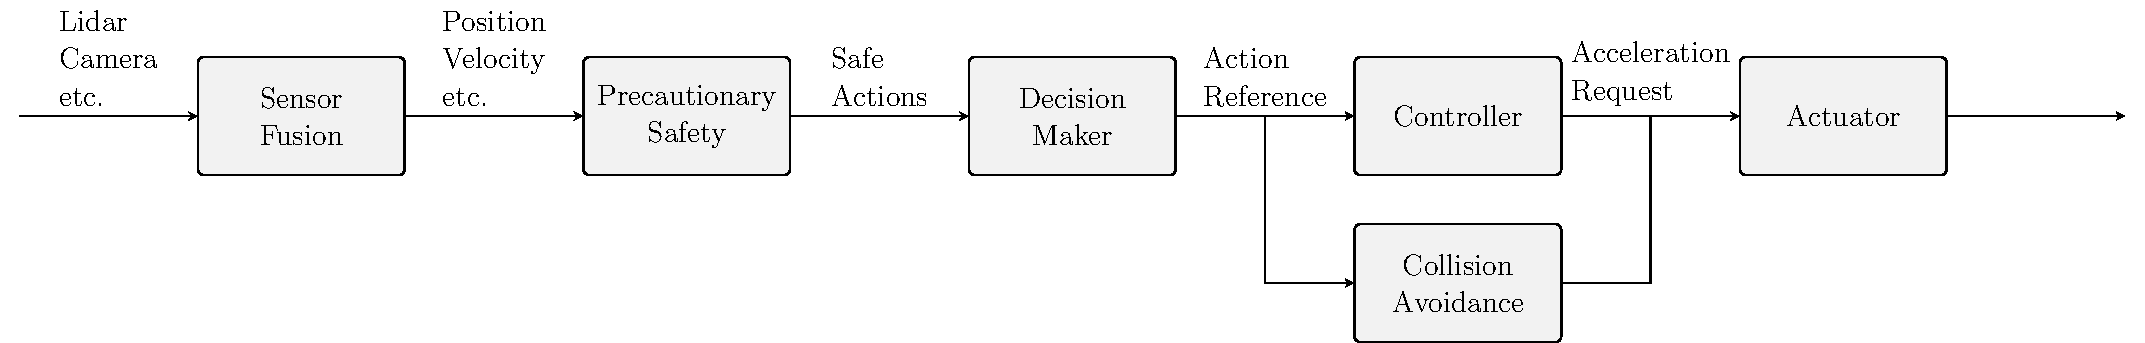
\includegraphics[width=\linewidth]{YourThesis/chapters/figures/pomdp/figures-system_architecture.pdf}
%	\begin{tikzpicture}[
%		node distance=8mm and 30mm,
%		node font= \Large,
%		box/.style = {draw, thick, rectangle, rounded corners=0.1cm, fill=gray!10, minimum width=3.5cm, minimum height=2cm, align=center},
%		sx+/.style = {xshift = 2mm},
%		sx+/.style = {xshift = 2mm}
%		]
%
%		% \node[draw,thick,rectangle,rounded corners =0.05cm,fill=gray!10,minimum width=2cm,minimum height = 2cm] (SF) at (2,0) {Sensor Fusion};
%		
%		% \draw[arrow,thick] (0,0) --(SF) node [midway,above] {Sensors: Lidar, Radar, Camera, Sonar};
%
%		% \node[draw,thick,rectangle,rounded corners =0.05cm,fill=gray!10,minimum width=2cm,minimum height = 2cm, shift={(2,0,0)}] (SF) at (2,0) {Sensor \\ Fusion};
%		
%		\node (start) at (0,0) {};
%		\node (SF) [box, right=of start.east] {Sensor \\ Fusion};
%		\node (PS) [box, right=of SF.east] {Precautionary \\ Safety};
%		\node (DM) [box, right=of PS.east] {Decision \\ Maker};
%		\node (Con) [box, right=of DM.east] {Controller};
%		\node (CA) [box, below=of Con] {Collision \\ Avoidance};
%		\node (Act) [box, right=of Con.east] {Actuator};
%		\node (end) [right=of Act] {};
%
%		\draw[arrow,thick,align=left] (start) --+(SF) node [midway,above] {Lidar\\Camera\\etc.};
%		\draw[arrow,thick,align=left] (SF) --+(PS) node [midway,above] {Position\\Velocity\\etc.};
%		\draw[arrow,thick,align=left] (PS) --+(DM) node [midway,above] {Safe\\Actions};
%		\draw[arrow,thick,align=left] (DM) --+(Con) node [midway,above] {Action\\Reference};
%		\draw[arrow,thick,align=left] (DM) -| ($(DM.east) + (1.5,0mm)$) |- (CA) node [midway,above] {};
%		\draw[arrow,thick,align=left] (CA) -| ($(CA.east) + (1.5,0mm)$) |- (Act) node [midway,above] {};
%		\draw[arrow,thick,align=left] (Con) --+(Act) node [midway,above] {Acceleration\\Request};
%		\draw[arrow,thick,align=left] (Act) --+(end) node [midway,above] {};
%	% --> Sensor Fusion --> Precautionary Safety --> |Decision Maker --> Controller |--> Actuator -->
%	% 																->Collision Avoidance |
%
%	\end{tikzpicture} 
	\caption{Representation of the system architecture.}
	\label{fig:system_architecture}
\end{figure}

Although safety is the most important requirement for enabling autonomous driving, the work in this paper does not make any safety guaranties. 
Instead, I proposed that the decision making algorithms presented in this paper are used in system architecture shown in Figure~\ref{fig:system_architecture}. This way, the higher \gls{asil} classifications are on the precautionary safety and collision avoidance modules while the decision makers mainly focus on comfort and the \gls{asil} classification could be on the lower levels and in the best case even be classified as QM. 

\tommy{To explore different ways to make the driving policy safe and increase the capability of handling uncertainty in the environment. But even so the state of machine learning and neural networks today is still very limited when its comes to guaranteeing safety. Therefore, it is important to have a system architecture that can separate safety guarantees to another module so that the main benefits of using machine learning can be fully utilized.}

% \tommy{To be able to use \gls{ml} and \gls{rl} safety is this stage of development it is important to separate the responsibility of safety to a more capable system like formal methods, reachability or MPC that can mathematically guarantee safety.}
 
% \tommy{depending on size of chapter consider moving it to its own chapter.}
 
% The ASIL assessed for a given hazard is then assigned to the safety goal set to address that hazard and is then inherited by the safety requirements derived from that goal.
% These Severity, Exposure, and Control definitions are informative, not prescriptive, and effectively leave some room for subjective variation or discretion between various automakers and component suppliers.



% This paper aims to sparate the task of ensuring safety to a precautionary safety or collision avoidance module. 

% \todo{include a description of ISO26262, motivate a redundant system for Asil D, making it important to separate the scope of the tactical decision making agent to be comfortable and efficient. Efficiency can be measured in different ways, but in this paper we refer to change in acceleration, number of times the agent reaches an undesired terminal state and the time it takes to reach the goal.}



\section{Research questions}
\label{sec:research_questions}
This thesis defines human driving as sequential decision making under uncertainty. Decisions such as overtaking a slow driver or when to cross an intersection are often made with limited information and some prediction estimate based on previous experience. 
This section briefly introduce the intersection problem, why its hard and the research questions that are studied in this paper. 
% A simple unsignalized intersection is shown in Figure \ref{fig:zones}.
In some cases like highway driving the uncertainty is very low, but when it comes to more urban environment this uncertainty increases. Compared to highway, urban environments introduce more uncertainty. 
Investigate how \gls{rl} methods can be used in practice to create a tactical decision making agent for \gls{ad}.

\tommy{This paper focus on the DQN algorithm and investigate how far we can push it for decision making}

\begin{enumerate}
	\item The goal for the ego vehicle is to drive through intersections without colliding. 
	\item The intersection can be of different shapes. %We assume we have a map of the intersection. 
	\item There will be other vehicles crossing the same intersection. 
	\item The intention of other drivers are not known
	
\end{enumerate}

The work presented in this thesis investigate the following research questions:
\begin{enumerate}
	\item[\textbf{Q1.}] How can RL be used to create a decision-making agent for autonomous driving through an  intersection?
	% \item[\textbf{Q1.}] How can RL be used to create a decision-making agent for autonomous driving, that can handle different unsignalized intersections (complex urban scenarios)? Learn a scalable policy that is able to handle different scenarios. Relative coordinate system. Action space. 
	% (specificera for att komma undan varfor har du inte kollat pa andra metoder. How can we use RL for AD )
	\item[\textbf{Q2.}] Can a good driving policy be found without explicitly predicting other drivers intentions?
	% \item[\textbf{Q2.}] Can we find a driving policy without explicitly predicting other drivers intentions?
	% LSTM or other netowrk structures can find the hidden state that is intention. 
	\item[\textbf{Q3.}] How can MPC be used to improve the action and state space for a RL agent? 
	% \item[\textbf{Q3.}] How can AD domain knowledge (and models) be used to improve the action and state space for a RL agent? MPC for actions, Particle filter for intention distribution. How can AD domain knowledge be used to create a state and action space that improves the RL agent?
	\item[\textbf{Q4.}] How can the quality of a RL agent be improved by accounting for uncertainty?
	% (How can the uncertainty of the RL agent be utilized?) (RPF-in the output and PF-in the input space)

	% \item[\textbf{Q5.}] Where does ML/RL fit in the system architecure for decision making?
	% (PAPER A shows that RL can make decisions that finds a gap inbetween cars, PAPER B found that we RL can learn the utility of different actions and decrease the computational power required by modeling and predicting each action in the MPC. While MPC can ganerate a safe path that guarantees safety.) 
\end{enumerate}

\section{Scope and limitations}
\label{sec:scope}
The following aspects of creating a tactical decision making agent for autonomous driving in uncertain environments are not considered in this thesis. 

\begin{enumerate}
	\item We have access to sensors on-board the ego vehicle. We do not have v2v, or v2x communication. 
	\item We do not assume any knowledge of traffic signs or traffic lights. 
	\item Do not guarantee safety, the best we can do its making the decisions not trigger collision avoidance functions. 
	\item The work in this thesis is tested in simulation environments and not real world. 
	\item This work considers the control of one vehicle and not multiple agents. 
	\item A reward function is defined for each approach. 
	
	To compensate for not having v2v or v2x communication, we have to, directly or indirectly, predict what other driver will do. 
	
\end{enumerate}


\section{Contributions}
\label{sec:contributions}
\todo{Rewrite once thesis is in a better state}
The main contributions of this thesis are:
\begin{enumerate}
	\item General approach to creating a decision making agent for driving in interactions. 
	\item A neural network architecture that is invariant to permutations of the order of which surrounding traffic participants are observed, which speeds up training and improves the quality of the trained agent. 
	\item REWRITE: A belief state representation using a particle filter and a comparison and analysis of different algorithms that utilize the belief state. 
	\item Two approached to solving a POMDP with hidden intention state. LSTM layer and belief state. 
	\item General state space representation that is invariat to permutations of the intersection design. 
	\item Extension of RL methods that provide an estimate of the epistemic uncertainty and use it to create a confidence criteria that can identify situations with high uncertainty. 
	\item \todo{Transfer reinforcement learning, finding a policy for mdps }

\end{enumerate}


\section{Thesis outline}
The outline of the thesis is as follows: in Chapter \ref{ch:related_work} other research in the same field is presented. In Chapter \ref{ch:background} introduce the mathematical framework \gls{mdp} and \gls{pomdp} with a brief theory of \gls{rl}. 
Chapter \ref{ch:modeling_intersection} is where the problem is formulated by defining the components of the \gls{pomdp}. In Chapter \ref{ch:mpc}, performance results from using deep Q-learning to solve the \gls{pomdp} is presented and later combined with a \gls{mpc} to improve the actions. Later in Chapter \ref{ch:uncertainty} two approaches to handle the uncertainty is presented. First the uncertainty in the decisions from the \gls{rl} algorithm and then an empirical study of how well a \gls{dqn} can handle uncertainty of others driving intentions. Chapter \ref{ch:generalize} present an approach to generalize over differnt \gls{mdp}s more specifically policies learned from different transfer functions. 


